\chapter{Cifras Clássicas}
\label{cha:cifras-classicas}

Como argumentamos no primeiro capítulo, a internet é um meio de comunicação promíscuo.
As partes que se comunicam pela rede não tem controle sobre por quais caminhos sua comunicação irá trafegar.
Essa característica, porém, não se restringe a esse meio.
Durante o século XVIII, por exemplo, toda correspondência que passava pelo serviço de correios de Viena na Austria era encaminhada para um escritório -- {\em black chamber} -- que derretia o selo, copiava seu conteúdo, recolocava o selo e reincaminhava para o destinatário.
Todo esse processo durava cerca de três horas para não atrasar a entrega.
Como a Áustria, todas as potências européias desse período operavam suas {\em back-chambers}.
As invenções do telegrafo e do rádio só facilitaram a capacidade de criar grampos, no primeiro caso, ou simplesmente captar a comunicação no segundo \cite{Kahn96}.

Partiremos, portanto, do seguinte modelo de comunicação.
Duas partes, o remetente e o destinatário, buscam se comunicar.
Tradicionalmente denominaremos o remetente de Alice e o destinatário de Bob.
Nossa suposição principal é que o canal de comunicação entre as partes é inseguro.
Ou seja, assumiremos que terceiros, que denominaremos de Eva, são capazes de observar as mensagens que trafegam pelo canal de comunicação.
Essa suposição é conhecida em alguns meios como ``hipótese da comunicação hacker''.
Para efeitos deste curso, sempre assumiremos essa hipótese.

A {\em criptografia} (do grego ``escrita secreta'') é a pratica e o estudo de técnicas de comunicação segura na presença de terceiros chamados de {\em adversários}.
Nosso primeiro desafio no curso é apresentar sistemas de comunicação que garantam a {\em confidencialidade}.
Ou seja, toda mensagem enviada de Alice para Bob deve ser compreensível apenas para Alice e Bob e deve ser incompreensível para Eva:
\begin{center}
\begin{tikzpicture}[node distance=2cm,auto,>=latex]
\node (alice) {Alice};
\node (bob) at (10,0) {Bob};
\node (eva) at (5,2) {Eva};
\draw[->] (alice) -> node[above]{mensagem} (bob);
\path[->] (eva) edge (5,.5);
\end{tikzpicture}
\end{center}

Se a importância da comunicação confidencial entre civis tem se tornado cada vez mais urgente, no meio militar é difícil remontar suas origens.
Suetônio (69 - 141) por volta de dois mil anos atrás descreveu como o imperador Júlio César (100 a.c. - 44 a.c.) escrevia mensagens confidenciais:


\begin{quote}
  ``Se ele tinha qualquer coisa confidencial a dizer, ele escrevia cifrado, isto é, mudando a ordem das letras do alfabeto, para que nenhuma palavra pudesse ser compreendida.
  Se alguém deseja decifrar a mensagem e entender seu significado, deve substituir a quarta letra do alfabeto, a saber 'D', por 'A', e assim por diante com as outras.''
\end{quote}

O esquema que chamaremos de cifra de César é ilustrado pelo seguinte exemplo:

\begin{verbatim}
Mensagem: transparenciapublicaopacidadeprivada
Cifra:    XUDQVSDUHQFLDSXEOLFDRSDFLGDGHSULYDGD
\end{verbatim}

Como descrito por Suetônio, a regra para encriptar uma mensagem consiste em substituir cada letra da mensagem por aquela que está três posições a sua frente na ordem alfabética.
Para descriptografar a cifra, substituir cada letra por aquela que está três posições atrás.
O problema com este tipo de sistema é que basta conhecer a regra de criptografia para decifrá-lo.
Em outras palavras, o segredo da cifra é sua própria regra.

Embora técnicas de criptografia e criptoanálise existam desde o império romano, foi com o advento do teléfgrafo e sua capacidade de comunicação eficiente, que o campo se estruturou.
No fim do século XIX Auguste Kerckhoff estabeleceu seis princípios que as cifras militares deveriam satisfazer:
\begin{enumerate}
\item O sistema deve ser indecifrável, se não matematicamente, pelo menos na prática.
\item O aparato não deve requerer sigilo e não deve ser um problema se ele cair nas mãos dos inimigos.
\item Deve ser possível memorizar uma chave sem ter que anotá-la e deve ser possível modificá-la se necessário.
\item Deve ser possível aplicar a sistemas telegráficos.
\item O aparato deve ser portátil e não deve necessitar de muitas pessoas para manipulá-lo e operá-lo.
\item Por fim, dadas as circunstâcias em que ele será usado, o sistema deve ser fácil de usar, não deve ser estressante usá-lo e não deve exigir que o usuário conheça e siga uma longa lista de regras.
\end{enumerate}

O segundo princípio ficou conhecido como {\em princípio de Kerckhoff}.
Ele estabelece que a regra usada para criptografar uma mensagem, mesmo que essa regra esteja codificada em um mecanismo, não deve ser um segredo e não deve ser um problema caso ela caia nas mãos do adversário.
Nas palavras de Claude Shannon: ``o inimigo conhece o sistema''.
Whitfield Diffie coloca o debate nos seguintes termos:

\begin{quote}
``Um segredo que não pode ser rapidamente modificado deve ser interpretado como uma vulnerabilidade''
\end{quote}

Ou seja, em uma comunicação confidencial as partes devem compartilhar algo que deve ser ``possível de modificar caso necessário''.
Esse segredo compartilhado é o que chamaremos de {\em chave} da comunicação e assumiremos que ela é a única parte sigilosa do sistema.
Trazendo o debate para uma discução mais moderna, o sigilo do código-fonte de um sistema não deve em hipótese alguma ser aquilo que garanta sua segurança.

O modelo de {\em criptografia simétrica}, portanto, pode ser descrito da seguite maneira:
o remetente usa um algoritmo público ($E$) que, dada uma chave ($k$), transforma uma mensagem ($m$) em um texto incompreensível chamado de {\em cifra} ($c$), a cifra é enviada para o destinatário por um meio assumidamente inseguro (hipótese da comunicação hacker) e o destinatário utiliza a mesma chave em um algoritmo ($D$) que recupera a mensagem a partir da cifra.

\begin{center}
\begin{tikzpicture}[node distance=2cm,auto,>=latex]
\node (alice) at (0, 2){Alice};
\node (bob) at (10, 2) {Bob};
\node (eva) at (5, 2) {Eva};

\node (m1) at (0,1) {$m$};
\node (k1) at (0,-1) {$k$};
\node (E)  at (2,0) {$E(k,m) = c$};
\node (D)  at (8,0) {$D(k,c) = m$};
\node (k2) at (10,-1) {$k$};
\node (m2) at (10,1) {$m$};

\path[->] (eva) edge (5,1);
\draw[->] (m1) -> (E);
\draw[->] (k1) -> (E);
\draw[->] (D) -> (m2);
\draw[->] (k2) -> (D);
\draw[->] (E) -> node[above]{$c$} (D);
\end{tikzpicture}
\end{center}

\section{Cifra de Deslocamento}
\label{sec:cifra-deslocamento}

O que chamamos na seção anterior como ``cifra de César'' não deve ser propriamente considerado uma cifra, pois não possui uma chave.
Porém, é possível e simples adaptar esse esquema para incorporar uma chave.
Para tanto faremos a seguinte alteração no esquema.
Ao invés de deslocar as letras sempre três casas para frente vamos assumir que foi sorteado previamente um número $k$ entre $0$ e $23$.
Esse número será a chave da comunicação e, portanto, assumiremos que as partes a compartilham.
O mecanismo para criptografar uma mensagem será o de deslocar cada letra $k$ posições para a direita e para descriptografá-la basta deslocar cada letra as mesmas $k$ posições para a esquerda.

Para formalizar este mecanismo vamos assumir que cada letra do alfabeto seja representada por um número: a letra {\tt a} será representada pelo $0$, a letra {\tt b} pelo $1$ e assim por diante.
O universo de todas as chaves possíveis é o conjunto $K = \{0 ... 23\}$ (chamaremos este conjunto de $\mathbb{Z}_{26}$ ou de maneira mais genérica $\mathbb{Z}_n = \{0, 1, \dots, n - 1\}$) e o universo de todas as mensagens possíveis é representado pelo conjunto $M = {\mathbb{Z}_{26}}^\star$, ou seja, todas as sequências de números entre $0$ e $23$.
Além disso, o conjunto das possíveis cifras é $C = M$.
Precisamos descrever três algorítmos:
\begin{itemize}
\item $Gen$ que gera a chave $k \in K$,
\item $E$ que recebe uma chave $k \in K$ e uma mensagem $m \in M$ e produz uma cifra $c \in C$ (i.e.: $E: K \times M \to C$) e
\item $D$ que recebe uma chave $k \in K$ e uma cifra $c \in C$ e produz uma mensagem $m \in M$ (i.e.; $D: K \times C \to M$).
\end{itemize}

Um sistema de criptografia simétrica $\Pi$ é formado por essa tripla de algoritmos $\Pi = \langle Gen, E, D \rangle$.
Além disso, precisamos garantir que quem possui a chave seja capaz de descriptografar a cifra.
Ou seja, precisamos garantir que:
\begin{displaymath}
  D(k, E(k, m)) = m
\end{displaymath}

O mecanismo que gera uma chave na cifra de substituição é bastante simples, ele simplesmente sorteia com uma distribuição de probabilidade uniforme um número entre $0$ e $23$.
Escreveremos da seguinte forma:
\begin{displaymath}
Gen := k \leftarrow \mathbb{Z}_{26}
\end{displaymath}

Utilizaremos a partir daqui a convenção de usar uma seta da direita para esquerda indicando que será escolhido um elemento do conjunto com probabilidade uniforme.

O algoritmo para criptografar uma mensagem traz um pequeno problema.
Escreveremos $m = m_0 m_1 m_2 \dots m_n$ uma mensagem $m$ com $n + 1$ letras cuja primeira letra é $m_0$, a segunda é $m_1$ e assim por diante.
Nossa primeira tentativa de formalizar $E$ seria somar $k$ a cada uma das letras $m_i$.
O problema é que esta soma pode resultar em um valor que não corresponde a nenhuma letra i.e. $m_i + k > 23$.
Para evitar este problema utilizaremos não a aritmética convencional, mas a {\em aritmética modular}.

Dizemos que um número $a$ divide $b$ (escrevemos $a|b$) se existe um número inteiro $n$ tal que $a.n = b$.
Dois números são equivalentes módulo $n$ (escrevemos $a \equiv b\ (mod\ n)$) se $n|(b-a)$.
Em outras palavras, dois números são equivalentes módulo $n$ se o resto da divisão de cada um por $n$ for o mesmo reultado.
O conjunto de todos os números equivalentes módulo $n$ forma uma classe de equivalência que representaremos como $[a\ mod\ n] = \{b \in \mathbb{Z} : a \equiv (b\ mod\ n)\}$.
Por exemplo $[5 + 7\ mod\ 10] = [2\ mod\ 10]$ pois $5 + 7 = 12$ e o resto de $12$ por $10$ é $2$.

Estamos finalmente em condições de formalizar o sistema da cifra de deslocamento $\Pi = \langle Gen, E, D\rangle$:
\begin{itemize}
\item $Gen := k \leftarrow \mathbb{Z}_{26}$
\item $E(k, m) = [m_0 + k\ mod\ 26] \dots [m_n + k\ mod\ 26]$
\item $D(k, c) = [c_0 - k\ mod\ 26] \dots [c_n - k\ mod\ 26]$
\end{itemize}


\begin{example}
  Considere a palavra {\tt XUXA}.
  Usando a cifra de César com chave $k = 3$ obtemos a cifra {\tt BZBD}.

  \begin{itemize}
  \item $E(3, \textrm{\tt 24 21 24 0}) = [1\ mod\ 26] [21\ mod\ 26] [1\ mod\ 26] [3\ mod\ 26]$
  \item $D(3, \textrm{\tt 1 21 1 3}) = [24\ mod\ 26] [21\ mod\ 26] [24\ mod\ 26] [0\ mod\ 26]$
  \end{itemize}

  Note que $[27\ mod\ 26] = [1\ mod\ 26]$ e que $[-2\ mod\ 26] = [24\ mod\ 26]$.
\end{example}



\section{Cifra de Substituição}
\label{sec:cifra-monoalfabetica}

Em 1567 a residência da rainha da Mary da Escócia foi destruída por uma explosão que levou a morte do então rei, primo de Mary.
O principal suspeito do assinato foi dispensado da pena e se casou com Mary no mês seguinte.
O episódio levou-a a prisão na Inglaterra.
Neste tempo, para a maioria dos católicos, Mary era a legítima herdeira do trono inglês - ocupado pela protestante Elizabeth I.
Durante o tempo na prisão Mary conspirou com aliados pela morte de Elizabeth.
Em 1587 Mary foi executada pelo que ficou conhecido como a conspiração de Babington.
A principal prova utilizada para a condenação foi uma troca de cartas cifradas interceptadas e decifradas \cite{Singh04}.

A cifra usada pelos conspiradores é conhecida hoje como {\em cifra de substituição} ou {\em cifra monoalfabética}.
Neste tipo de criptografia, cada letra ou par de letras é substituída por um símbolo, que pode ser inclusive uma outra letra.
Assim, a chave desse tipo de cifra é um alfabeto.


\begin{example}
  Considere a seguinte chave de uma cifra monoalfabética.
  Neste caso os símbolos utilizados letras do mesmo alfabeto em ordem embaralhada:
  \begin{verbatim}
    Alfabeto:   abcdefghijklmnopqrstuvwxyz
    Permutação: ZEBRASCDFGHIJKLMNOPQTUVWXY
  \end{verbatim}

  A partir desta chave podemos produzir textos substituindo cada letra pela letra correspondente na chave.
  Para descriptografar, basta fazer o processo inverso, a saber, substituir a letra da cifra pela do alfabeto.

  \begin{verbatim}
    Mensagem: transparenciapublicaopacidadeprivada
    Cifra:    QOZKPMZOAKBFZMTEIFBZLMZBFRZRAMOFUZRZ
  \end{verbatim}
\end{example}

O desfecho da história da conspiração de Babington sugere que a cifra monoalfabética não é muito segura.
De fato, no próximo capítulo discutiremos melhor as técnicas de criptonálise para este tipo de cifra.
Não obstante, até o desenvolvimento das primeiras máquinas de criptografar, versões das cifras monoalfabéticas eram as cifras mais populares no mundo todo.
Nos anos 70 a editora abril publicou no Brasil o famoso Manual do Escoteiro Mirim da Disney que apresentava uma cifra monoalfabética.
Mais recentemente, o curioso caso do desaparecimento de um rapaz no Acre viralizou quando seus familiares revelaram que no seu quarto havia uma coleção de livros que ele havia escrito de maneira criptografada.
Mais tarde foi descoberto que o rapaz usara uma cifra de substituição cuja chave foi eventualmente encontrada.

Para fechar esta seção buscaremos formalizar o sistema de cifra de substituição simples.
Uma {\em permutação} sobre um conjunto $\Sigma$ qualquer é uma {\em função bijetora} $p: \Sigma \to \Sigma$.
Funções bijetoras possuem a característica de serem inversíveis, ou seja, existe $q: \Sigma \to \Sigma$ tal que $p(q(x)) = q(p(x)) = x$.
A função $q$ é chamada de {\em inversa} de $p$, é única e será representada como $p^{-1}$.
O conjunto de todas as permutações, todas as funções bijetoras, de $\Sigma$ será representado como $Perm(\Sigma)$.
A chave de uma cifra de substituição é uma permutação do alfabeto $\mathbb{Z}_{26}$ escolhida aleatoriamente.
Para encriptar uma mensagem basta aplicar essa permutação a cada uma das mensagens e para descriptografá-la basta aplicar a função inversa.

Formalmente temos que $\Pi = \langle Gen, E, D \rangle$ em que:
\begin{itemize}
\item $Gen := k \leftarrow Perm(\mathbb{Z}_{26})$
\item $E(k, m) = k(m_0) \dots k(m_n)$
\item $D(k, c) = k^{-1}(c_0) \dots k^{-1}(c_n)$
\end{itemize}

\section{Cifra de Vigenère}
\label{sec:cifra-de-vigenere}

A cifra de Vigènere foi criada no século XV e ainda no começo do século XX era considerada inquebrável -- em 1868 o matemático e autor de Alice no País das Maravilhas, descreveu a cifra como ``inquebrável'' e um artigo da Scientific American de 1917 a descrevia como ``impossível de traduzir''.
Veremos no próximo capítulo que há um exagero nessas descrições, porém, a sofisticação desse tipo de cifra chamado de {\em polialfabética} tornava sua criptoanálise muito mais sofisticado.

Em poucas palavras, a cifra de Vigenère consiste em deslocar as letras do texto original em distâncias diferentes.
Em sua versão mais simples, sua chave consiste de uma palavra cuja primeira letra indica quantas casas devemos deslocar a primeira letra da mensagem, a segunda letra da chave indica quantas casa devemos deslocar a segunda letra e assim por diante.
Quando a mensagem ultrapassa o tamanho da chave, repetimos a chave e continuamos o processo.

Para facilitar a conta na hora de criptografar e descriptografar, podemos usar uma tabela que indica para cada letra da mensagem e cada letra da chave qual é a letra correspondente na cifra.
Essa tabela é chamada de {\em tabula recta} e está representada na Figura \ref{fig:tabula-recta}.

\begin{figure}[htbp]
  \centering
  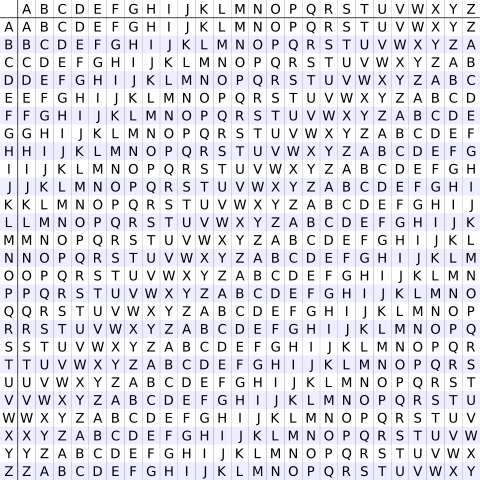
\includegraphics[width=.8\textwidth]{imagens/tabula-recta.png}
  \caption{Tabula Recta}
  \label{fig:tabula-recta}
\end{figure}


\begin{example}
  Considere a seguinte mensagem criptografada com a chave {\tt senha} usando a cifra de Vigenère:

\begin{verbatim}
Mensagem: transparenciapublicaopacidadeprivada
Chave:    senhasenhasenhasenhasenhasenhasenhas
Cifra:    LVNUSHEELNUMNWUTHVJAGTNJIVEQKPJMIHDS
\end{verbatim}
\end{example}

Para fechar o capítulo vamos fazer o exercício de formalizar a cifra de Vigenère.
A chave consiste em uma sequência de letras, tipicamente escolhidas em um dicionário, mas vamos aqui supor que a escolha seja aleatória e com um tamanho fixado $l$.
Para criptografar basta desolcar $m_i$ por $k_{[i\ mod\ n]}$ posições.
Formalmente temos que $\Pi = \langle Gen, E, D \rangle$

\begin{itemize}
\item $Gen := k \leftarrow \mathbb{Z}_{26}^l$
\item $E(k, m) = [m_0 + k_{[0\ mod\ l]}\ mod\ 26] \dots [m_n + k_{[n\ mod\ l]}\ mod\ 26]$
\item $D(k, c) = [c_0 - k_{[0\ mod\ l]}\ mod\ 26] \dots [c_n - k_{[n\ mod\ l]}\ mod\ 26]$
\end{itemize}

\section{Máquinas de Criptografar}
\label{sec:maquinas}

No final da primeira década do século XX foram inventadas as primeiras máquinas de criptografar.
A componente principal dessas {\em maquinas eletromecânicas} é um conjunto de {\em rotores}.
A configuração inicial dos rotores contém a chave da criptografia.
Cada vez que o operador pressiona uma tecla o rotor embaralha as letras.
Dessa forma, essas {\em máquinas rotoras} se comportam como uma sofisticada cifra polialfabética.
Para descriptografar a mensagem, o operador precisa ajustar a máquina em modo de descriptografia, ajustar a configuração inicial com a chave secreta e digitar o texto cifrado.
A máquina então irá se rearrajar para produzir o texto original quando digitado.

As máquinas rotoras mais conhecidas são da série {\em Enigma}.
Elas foram criadas por um inventor alemão no final da primeira guerra mundial e versões mais modernas foram extensamente usadas durante a segunda guerra pelo exército nazista.
As versões mais simples da máquina possuiam três rotores capazes de gerar $26^3 \approx 17.500$ possíveis configurações iniciais.
Além disso, era possível trocar a ordem dos rotores multiplicando por $6$ o número de combinações possíveis, chegando a um total de cerca de $105$ mil possibilidades.
A versão utilizada pelo exercito nazista, porém, permitia cerca de $150$ trilhões de possibilidades.
Em 1939 Alan Turing desenvolveu uma máquina eletromecânica chamada {\em Bombe} capaz de decifrar algumas cifras de máquinas Enigma com 3 rotores e, posteriormente foi melhorada para decifrar mensagens de máquinas Enigma mais sofisticadas.

A história da computação esbarra na história da criptografia neste ponto.
Poucos anos antes da guerra, Alan Turing demonstrara que a satisfatibilidade da lógica de primeira ordem é um {\em problema indecidível}.
Para tanto ele propôs um {\em modelo computacional} que hoje chamamos de {\em Máquinas de Turing}.
Diferente dos modelos computacionais anteriores como o {\em cálculo lambda} de Church ou as {\em funções recursivas} de Gödel, o modelo de Turing era intuitivo.
Além disso, Turing mostrou que era possível construir com seu modelo uma {\em Máquina Universal} capaz de simular qualquer outra Máquina de Turing.
Esse resultado magnífico é o que dá origem a computação.
O primeiro modelo de computador desenvolvido por Turing e sua equipe em Bechley Park foi batizado de {\em Colossus} e tinha como principal propósito quebrar outra cifra usada pelos nazistas durante a guerra, a {\em cifra de Lorenz}.
A cifra de Lorenz é uma versão do que estudaremos com o nome de {\em cifra de fluxo}.
Para decifrar os códigos das máquinas Enigma e da cifra de Lorenz os ingleses tiveram que contar, não apenas com o texto criptografado que interceptavam sem grandes dificuldades, mas também com uma série de cifras cujas mensagens eles conheciam previamente.
Veremos mais pra frente a importância desta informação.
A capacidade dos aliados de decifrar as mensagens de seus adversários foi central para sua vitória.

O começo do século XX marcou o surgimento das primeiras máquinas de criptografar, as primeiras máquinas de criptoanálise.
Na metade do século começaram a surgir os primeiros computadores.
Nos anos 70 a comunicação seria revolucionada pelo advento da internet, mas antes disso já ficara claro que era necessário compreender melhor o que faz uma cifra ser segura.


\section{Criptoanálise}
\label{sec:criptoanalise}

Nos capítulos anteriores vimos uma série de cifras que a história deu conta de mostrar que não são seguras.
Neste capítulo focaremos nas técnicas para quebrar essas cifras.
O estudo e a análise dos sistemas de informação com a intenção de desvelar seus segredos é o que chamamos de {\em criptoanálise}.

\subsection{Ataques Força Bruta}
\label{sec:forca-bruta}

Uma forma universal de quebrar uma cifra é conhecido como {\em ataque força bruta}.
Ele consiste no seguinte procedimento.
O adversário utiliza o esquema $D$, que sempre assumimos ser de conhecimento público, numa cifra $c$ com uma primeira tentativa de chave $k_0$ para produzir $D(k_0, c) = m_0$.
A mensagem $m_0$ provavelmente não fará nenhum sentido, então o adversário repete o processo com uma outra chave $k_1$ e em seguida com $k_2$ e assim por diante até que mensagem produzida seja coerente.

Consideremos a cifra de deslocamento.
Estabelecemos que uma chave nesse tipo de sistema é escolhida aleatoriamente no conjunto $\mathbb{Z}_{26}$.
Assim existem exatamente 26 possibilidades de chave, porque $|\mathbb{Z}_{26}| = 26$.
O número esperado de tentativas até se encontrar a chave procurada é $\frac{|K|}{2}$, neste caso 13.
Ou seja, a cifra de deslocamento é muito vulnerável a ataques de força bruta porque seu universo de chaves é extremamente pequeno.

Em contraste vamos calcular o universo de chaves da cifra de substituição.
Vimos que o universo das chaves de uma cifra de susbstituição é $Perm(\mathbb{Z}_{26})$.
Calcular $|Perm(\mathbb{Z}_{26})|$ é um exercício simples de {\em análise combinatória}.

\begin{eqnarray*}
  |Perm(\mathbb{Z}_{26}|) & = & 26!\\
                         & = & 26.25.24 \dots 1\\
                         & \approx & 4.10^{26}\\
                         & \approx & 2^{88}
\end{eqnarray*}

O universo de chaves na cifra de deslocamento é tão pequeno que é possível testar na mão todas as possibilidades de chaves.
Certamente não é possível testar as possibilidades de chaves da cifra de substituição na mão.
Ataques força bruta, porém, são facilmente automatizáveis.
Voltaremos a pergunta sobre o tamanho do universo de chaves para uma comunicação segura no capítulo \ref{chap:senhas}.


\begin{example}
Muitos dos roteadores modernos possuem um mecanismo chamado de WPS (Wi-Fi Protected Setup) que supostamente simplificaria o processo de conexão, especialmente na configuração do hardware.
O WPS permite que um usuário se conecte remotamente e sem fio no roteador desde que possua um PIN (Personal Identification Number).
Esse PIN é uma sequência de oito digitos de 0 a 9.
Ou seja, o universo das chaves é $10^8 \approx 2^{27}$.
Neste contexto, um ataque força-bruta é possível e toma entre 4 e 8 horas.
\end{example}


\subsection{Ataques de Frequência}
\label{sec:frequencia}

A cifra de substituição é suficientemente segura contra ataques de força-bruta.
Como vimos, porém, ela não é tão segura quanto a rainha Mary da Escócia gostaria.
A forma como os funcionários da rainha Elizabeth quebraram a cifra de substituição é o que chamamos de {\em ataque de frequência}.
A ideia por trás desse tipo de ataque é bastante simples.
Na cifra de substituição, cada letra é substituída por um símbolo.
Portanto, a frequência de cada símbolo em um texto suficientemente longo deve ser parecida com a frequência média de cada letra naquela língua.
Por exemplo, no português, esperamos que os símbolos mais comuns sejam o {\tt a}, o {\tt e} e o {\tt o}.
Para piorar -- ou melhorar dependendo da perspectiva -- na maioria das línguas há digrafos particulares, por exemplo, no português dois símbolos repetídos provavelmente representam o {\tt r} ou o {\tt s} e o {\tt h} quase sempre vem depois do {\tt l} ou do {\tt n}.
Se o texto a ser decifrado for suficientemente longo, essas pistas podem ser suficientes para quebrar a cifra.

No seguinte trecho de ``O escaravelho de ouro'' de Edgar Allan Poe a personagem descreve essa técnica que ela utilizou para decifrar um texto em inglês \cite{}:

\begin{quote}
``Ora, no inglês, a letra que ocorre com mais frequência é a letra {\tt e}.
Depois dela, a sucessão é: {\tt a o i d h n r s t u y c f g l m w b k p q x z}.
O e prevalece de tal maneira que quase nunca se vê uma frase isolada em que ele não seja predominante.
Aqui nós temos, portanto, bem no início, uma base que permite mais do que um mero palpite.
O uso que se pode fazer da tabela é óbvio, mas, neste criptograma em particular, não precisamos nos valer dela por inteiro.
Como nosso caractere dominante é o {\tt 8}, começaremos assumindo que este é o {\tt e} do alfabeto normal. (...)''
\end{quote}

Em português, faz sentido separar as letras em cinco blocos, com frequência de ocorrência decrescente:
\begin{enumerate}
\item {\tt a}, {\tt e} e {\tt o}
\item {\tt s}, {\tt r} e {\tt i}
\item {\tt n}, {\tt d}, {\tt m}, {\tt u}, {\tt t} e {\tt c}
\item {\tt l}, {\tt p}, {\tt v}, {\tt g}, {\tt h}, {\tt q}, {\tt b} e {\tt f}
\item {\tt z}, {\tt j}, {\tt x}, {\tt k}, {\tt w} e {\tt y}
\end{enumerate}

\subsection{Ataques à ``Cifra Invencível''}
\label{sec:criptoanalise-vegenere}

Apesar da fama de ``inquebrável'' que a cifra de Vigenère ostentou até o começo do século XX, desde a metade do século anterior já eram conhecidos métodos de criptoanálise capazes de derrotar esse tipo de cifra.

Em 1854 John Hall Brock Thwaites submeteu um texto cifrado utilizando uma cifra supostamente por ele inventada.
Charles Babbage, o inventor das máquinas que precederam o computador moderno, mostrou que no fundo a cifra de Thwaites era equivalente a cifra de Vigenère.
Após ser desafiado, Babbage, decifrou uma mensagem criptografada por Thwaites duas vezes com chaves diferentes.

Em 1863 Friedrich Kasiski formalizou um ataque contra a cifra de Vigenère que ficou conhecido como {\em teste de Kasiski}.
O ataque considera o fato de que a chave se repete com uma frequência fixa e, portanto, há uma probabilidade de produzir padrões reconhecíveis.
Considere o exemplo extraído da Wikipédia:

\begin{example}
\begin{verbatim}
Mensagem: cryptoisshortforcryptography
Chave:    abcdabcdabcdabcdabcdabcdabcd
Cifra:    CSASTPKVSIQUTGQUCSASTPIUAQJB
\end{verbatim}
\end{example}

Note que o padrão CSASTP se repete na cifra.
Isso ocorre porque o prefixo {\tt crypto} foi criptografado com a mesma chave.
Uma vez encontrado um padrão como este, é calculada a distância entre as repetições.
Neste caso a distância é 16, o que significa que o tamanho da chave deve ser um divisor de 16 (2, 4, 8 ou 16).
Com esta informação, podemos aplicar um ataque de frequência nos caracteres de 2 a 2, de 4 a 4, de 8 a 8 e de 16 a 16.



\section{Exercício}
\label{sec:exercicio}

\begin{exercicio}
  Considere a seguinte mensagem:
  \begin{verbatim}
    privacidadepublicatranparenciaprivada
  \end{verbatim}
  \begin{itemize}
  \item Criptografe essa mensagem utilizando a cifra de deslocamento com $k = 3$.
  \item Criptografe essa mensagem utilizando a cifra de substituição com a seguinte permutação de letras: {\tt ZEBRASCDFGHIJKLMNOPQTUVWXY}
  \item Criptografe essa mensagem utilizando a cifra de Vigenère com chave {\tt senha}.
  \end{itemize}
\end{exercicio}

%\begin{exercicio}
  % Dá uma cifra e três chaves e pede para descriptografar?
%\end{exercicio}

\begin{exercicio}
  Mostre que a operação de adição $+$ modulo $n$ é um {\em anel} para qualquer valor de $n$.
Ou seja, para qualquer $a, b, c, n \in \mathbb{Z}$ temos que:
\begin{itemize}
\item {\em associatividade}: $(a+b)+c \equiv a+(b+c)\ mod\ n$ e $(ab)c \equiv a(bc)\ mod\ n$
\item {\em elemento neutro}: $a + 0 \equiv a\ mod\ n$ e $a.1 \equiv a\ mod\ n$
\item {\em inverso}: existe $-a$ tal que $a + (-a) \equiv 0\ mod\ n$
\item {\em distributividade}: $a(b + c) \equiv ab + ac\ mod\ n$
\end{itemize}
\end{exercicio}

\begin{exercicio}
  Mostre que se $n|a$ e $n|b$ então $n|(ra + sb)$ para quaisquer $r, s \in \mathbb{Z}$.
\end{exercicio}

\begin{exercicio}
  Dizemos que $a$ é o {\em inverso multiplicativo} de $b$ em $\mathbb{Z}_n$ sse $ab \equiv 1\ mod\ n$.
\begin{itemize}
\item Mostre que $2$ é o inverso multiplicativo de $5$ em $\mathbb{Z}_9$.
\item Mostre que $6$ não possui inverso multiplicativo em $\mathbb{Z}_{12}$
\end{itemize}
\end{exercicio}

\begin{exercicio}
  Proponha um sistema de criptografia simétrica e argumente porque ele é mais seguro do que os sistemas que vimos até aqui.
\end{exercicio}

\begin{exercicio}
Calcule o tamanho do universo das chaves em uma cifra de Vigenère da forma como usada normalmente (escolhendo um palavra) e na forma como apresentamos formalmente (sequência aleatória com tamanho fixo $l$)?
\end{exercicio}


\begin{exercicio}
Construa um script que extraia um corpus do português moderno (por exemplo, textos da wikipedia) e calcule a frequência de ocorrência das letras do alfabeto.
\end{exercicio}

\begin{exercicio}
Em 2017 um rapaz que ficou conhecido como menino do Acre ficou dias desaparecido e deixou uma serie de livros criptografados com cifra de substituição em seu quarto.
Na Figura \ref{fig:menino-do-acre} está reproduzida uma página de um desses livros.
Utilize a análise de frequência para decifrar o texto.
\end{exercicio}

\begin{figure}[htbp]
  \centering
  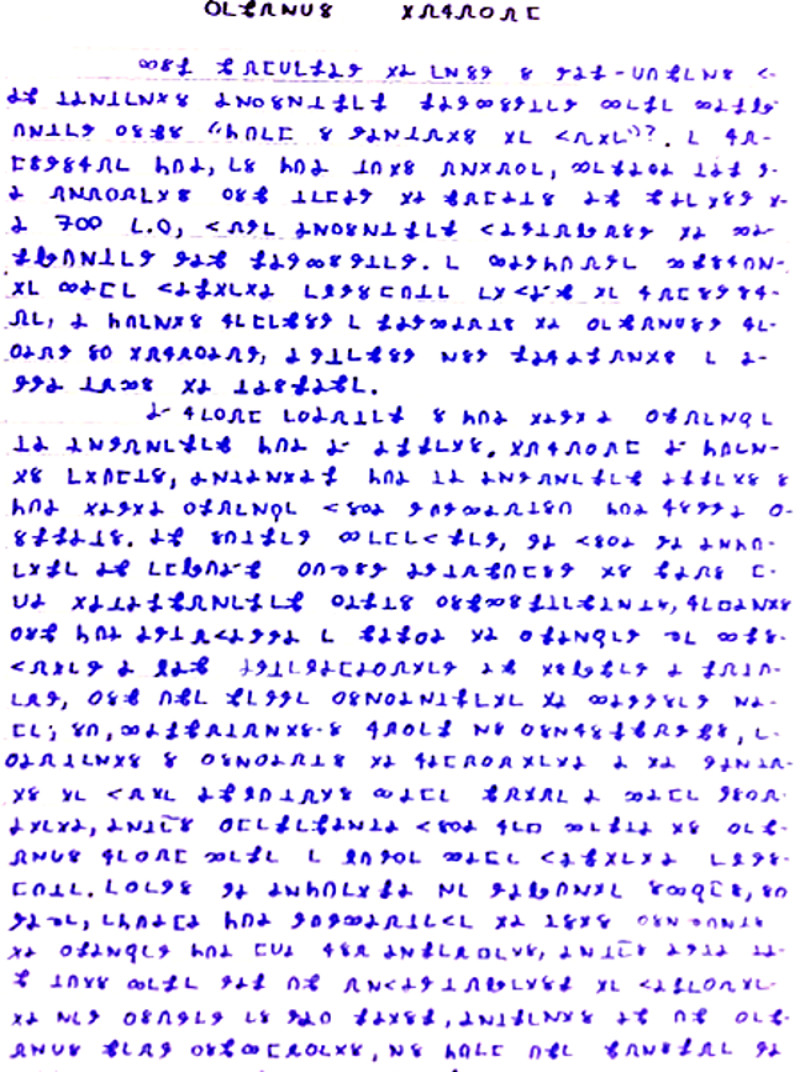
\includegraphics[width=.8\textwidth]{imagens/bruno.jpg}
  \caption{Texto criptografado pelo Menino do Acre}
  \label{fig:menino-do-acre}
\end{figure}
